\documentclass[12pt,a4paper,utf8x]{report}
\usepackage [frenchb]{babel}
\usepackage[pdftex]{graphicx}
%\usepackage{path}
% Pour pouvoir utiliser 
\usepackage{ucs}
\usepackage[utf8x]{inputenc}

\usepackage{url} % Pour avoir de belles url
\usepackage {geometry}

% Pour mettre du code source
\usepackage {listings}
% Pour pouvoir passer en paysage
\usepackage{lscape}

% Pour pouvoir faire plusieurs colonnes
\usepackage {multicol}
% POur crééer un index
\usepackage{makeidx}
\usepackage{color}

\usepackage{hyperref}
\usepackage{pdfpages}

\hypersetup{
    bookmarks=true,         % show bookmarks bar?
    unicode=false,          % non-Latin characters in Acrobat’s bookmarks
    pdftoolbar=true,        % show Acrobat’s toolbar?
    pdfmenubar=true,        % show Acrobat’s menu?
    pdffitwindow=false,     % window fit to page when opened
    pdfstartview={FitH},    % fits the width of the page to the window
    pdftitle={Documentation du flux},    % title
    pdfauthor={AUREGAN Pascal},     % author
    pdfsubject={Documentation du flux},   % subject of the document
    pdfcreator={AUREGAN Pascal},   % creator of the document
    pdfproducer={pdflatex}, % producer of the document
    pdfkeywords={keywords}, % list of keywords
    pdfnewwindow=true,      % links in new window
    colorlinks=true,       % false: boxed links; true: colored links
    linkcolor=Ror,          % color of internal links
    citecolor=green,        % color of links to bibliography
    filecolor=Ror,      % color of file links
    urlcolor=Ror           % color of external links
}
%fonte computer modern sans seriff

%\usepackage[T1]{fontenc}
%\usepackage{cmss}
%\newcommand\sfdefault{cmss}
\definecolor{Dark}{gray}{.2}
\definecolor{Medium}{gray}{.6}
\definecolor{Light}{gray}{.8}
\definecolor{Ror}{rgb}{0.65, 0.16, 0.16}

\newcommand*{\plogo}{
\includegraphics[clip=true, width=40mm, height=20mm]{./images/logo.jpg}}
%
\includegraphics[\textwidth,\textheight]{./images/logo.eps}
%pour une boite de couleur avec un texte de couleur
\newcommand{\boitecolor}[3]    {\colorbox{#1}{\textcolor{#2}{#3}}}

%\renewcommand{\paragraph}{\@startsection{paragraph}{4}{\z@}%
%            {-2.5ex\@plus -1ex \@minus -.25ex}%
%            {1.25ex \@plus .25ex}%
%            {\normalfont\normalsize\bfseries}}
            
%redefinition de la date
\date{	
	\normalsize{Lieu du stage\\
		Adresse du stage\\
		Ville du stage\\ 
		\vspace{5mm}	
		Directeur de recherche : M. DUPONT \\
		Rapporteur universitaire : Mme DUPUIS
	}
}

%Pour le titre joli
\newcommand*{\titleTH}{\begingroup% T&H Typography
	\protect\thispagestyle{empty}
	\begin{changemargin}{-2.5cm}{-1cm}
		\raggedleft
%		\vspace*{\baselineskip}
		{\Large Conservatoire National des Arts et Métiers}\\{\small Pascal AUREGAN}\\[0.167\textheight]

		{\bfseries Rapport de projet}\\[\baselineskip]
	%\end{changemargin}

%	\setlength{\textwidth}{208mm}
%	\begin{changemargin}{-2.5cm}{-1cm}
		\boitecolor{Ror}{white}{
			\makebox[208mm][r]{
				\Huge \textsf{NFE211}
		 }}\\[\baselineskip]
		%{\small illustrée}\par
		{\bfseries Test de chaine décisionnelle sur cas simple. }\\
		{\bfseries Base opérationnelle en fichier et PostgresSQL}\\
		{\bfseries ETL avec TALEND Data Integration,}\\
		{\bfseries Reporting avec SAS}\\
		\vfill

		{\Large \plogo}\par
		\vspace*{3\baselineskip}
	\end{changemargin}

	\pagebreak 
\endgroup}





\makeindex

% Pour les entetes de page

% \usepackage{fancyheadings}
%\pagestyle{fancy}
%\renewcommand{\sectionmark}[1]{\markboth{#1}{}} 
%\renewcommand{\subsectionmark}[1]{\markright{#1}} 

% Pour l'interligne de 1.5
\usepackage {setspace}
% Pour les marges de la page
\geometry{a4paper, top=2.5cm, bottom=3.5cm, left=2.5cm, right=1.5cm, marginparwidth=1.2cm}

\parskip=5pt %% distance entre § (paragraphe)
\sloppy %% respecter toujours la marge de droite 

% Pour les pénalités :
\interfootnotelinepenalty=150 %note de bas de page
\widowpenalty=150 %% veuves et orphelines
\clubpenalty=150 

%Pour la longueur de l'indentation des paragraphes
\setlength{\parindent}{15mm}



%%%% debut macro pour enlever le nom chapitre %%%%
\makeatletter
\def\@makechapterhead#1{%
  \vspace*{50\p@}%
  {\parindent \z@ \raggedright \normalfont
    \interlinepenalty\@M
    \ifnum \c@secnumdepth >\m@ne
        \Huge\bfseries \thechapter\quad
    \fi
    \Huge \bfseries #1\par\nobreak
    \vskip 40\p@
  }}

\def\@makeschapterhead#1{%
  \vspace*{50\p@}%
  {\parindent \z@ \raggedright
    \normalfont
    \interlinepenalty\@M
    \Huge \bfseries  #1\par\nobreak
    \vskip 40\p@
  }}
%
%\def\addcontentsline@toc#1#2#3{%
 % \addtocontents{#1}{\protect\thispagestyle{empty}}%
%   \addtocontents{#1}{\protect\contentsline{#2}{#3}{\thepage}}}
%\def\addcontentsline#1#2#3{%
 % \expandafter\@ifundefined{addcontentsline@#1}%
 % {\addtocontents{#1}{\protect\contentsline{#2}{#3}{\thepage}}}
 % {\csname addcontentsline@#1\endcsname{#1}{#2}{#3}}}

\makeatother
%%%% fin macro %%%%

%%%% debut macro %%%%
\newenvironment{changemargin}[2]{\begin{list}{}{%
\setlength{\topsep}{0pt}%
\setlength{\leftmargin}{0pt}%
\setlength{\rightmargin}{0pt}%
\setlength{\listparindent}{\parindent}%
\setlength{\itemindent}{\parindent}%
\setlength{\parsep}{0pt plus 1pt}%
\addtolength{\leftmargin}{#1}%
\addtolength{\rightmargin}{#2}%
}\item }{\end{list}}
%%%% fin macro %%%%

%Couverture 

\title
{
	\normalsize{DESS Xxxxx xxxx xxxxx\\
	Université de Xxxx Xxxxxx\\
	2004-2005}\\
	\vspace{15mm}
	\Huge{Titre du rapport de stage}
}
\author{Nom Auteur\\
	\vspace{45mm}
}



\renewcommand{\familydefault}{\sfdefault}
\begin{document}

%\setlength{\hoffset}{-1.5cm}
%\addtolength{\textwidth}{1cm}

\titleTH




%\setlength{\hoffset}{-1.5cm}


	\tableofcontents
	\clearpage

	% Pour avoir un interligne de 1,5
	\begin{onehalfspace}

		\chapter{Introduction}

Le but de se projet est de mettre en place une chaine décisionnelle. L'objectif de ce projet n'étant pas de pousser dans ses retranchements les outils de la chaine décisionnelle, il a été décidé de créer de toute pièce un jeu de données. Le thème de ce jeu de données est l'achat de BD comme dans le cours. 
La base opérationnelle décrit les factures d'un ensemble librairies en France dont les clients sont connus.
La chaine décisionnelle doit être en mesure de répondre in fine à la question: analyser les ventes de BD en France en fonction des clients, du lieu et date d'achat.
La couche opérationnelle est assurée par une base de données de fichier csv et une base de données PostgresSQL. 

Pour la couche ETL, il a été choisi TALEND Data Integration. 

La couche reporting étudiée lors de ce projet est assurée par SAS Studio Version Etudiante.

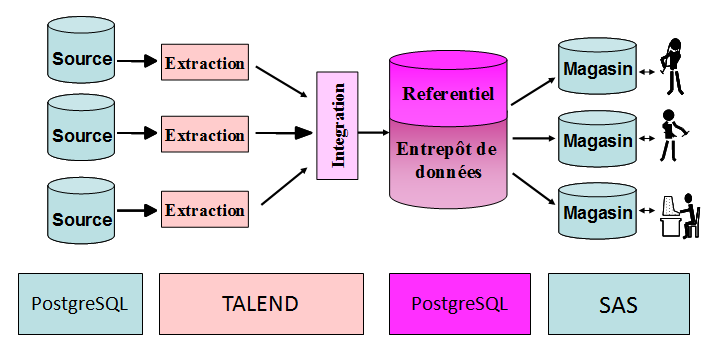
\includegraphics[clip=true, width=120mm, height=80mm]{images/chaine.png} 

\clearpage


		
\chapter{Jeu de données de la base OLTP}
\section{Modèle relationnel}
\subsection{Présentation}

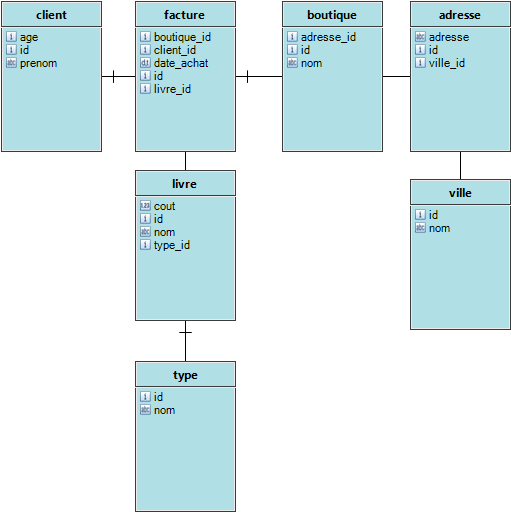
\includegraphics[clip=true, width=120mm, height=80mm]{./images/library.png}

Le modèle relationnel est un modèle normalisé. 
\begin{itemize}
\item Une facture a été établie pour un client donné dans une boutique donnée à une date donnée et en rapport avec un livre donné. 
\item Le livre appartient à un type donné (Roman, BD, etc.). 
\item La boutique a une adresse située dans une ville
\end{itemize}


Voici combien de lignes ont chaque table :
\begin{itemize}
\item adresse : 26
\item boutique : 25
\item client : 8819
\item facture : 8819
\item livre : 8
\item type : 3
\end{itemize}


En annexe, le code R qui a servi à générer les données dont il a été estimé que la pertinence n'avait que peu d'importance pour l'exercice.
De plus, nous possédons un fichier de type csv contenant un dictionnaire de villes avec les départements associés ainsi que les régions.
Voici en exemple les quatre premières lignes de ce fichier villes\_def.csv

\lstset{language=bash}
\lstset{frame=shadowbox}
\begin{lstlisting}
 "ville","departement","region_name"
 "Beauvais","Oise","Picardie"
 "Compiegne","Oise","Picardie"
 "Clermont","Oise","Picardie"
\end{lstlisting}

\clearpage




		
\chapter{TALEND Open Studio for Data Integration 5.6}

\section{Création du modèle OLAP}
\subsection{Question à répondre}
Analyse des ventes de bande dessinées d'une enseigne de librairie possédant plusieurs boutiques dans plusieurs villes.

\subsection{Modèle ROLAP}

L'implémentation ROLAP a été choisie par rapport au modèle MOLAP car même si la quantité de données était petite, il m'a semblé important d'étudier ce modèle qui paraît être très utilisé. Ne voyant rien justifier un modèle en flocon permettant de gagner de l'espace de stockage, j'ai utilisé un modèle en étoile.
La table de faits est la table vente. Les dimentsions sont le temps, la boutique(lieu d'achat), le client, et le livre. L'étoile est de type transaction.

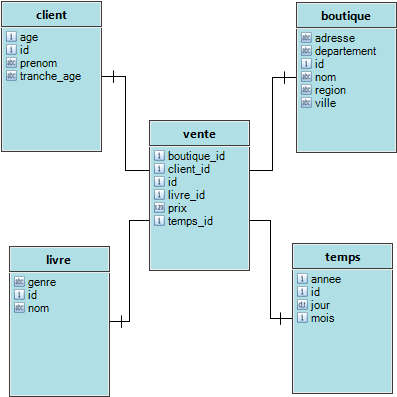
\includegraphics[clip=true, width=120mm, height=80mm]{images/Talend.png} 



\subsubsection{Table de faits vente}

\paragraph{Indicateurs}

prix de la vente; ce que le vente a rapporté

\subparagraph{fonctions d'agrégat}
\begin{itemize}
\item addition sur le prix
\item moyenne sur le prix
\end{itemize}


\paragraph{Dimension client}

\begin{itemize}
\item id
\item prenom
\item age
\item tranche\_age ("-12", "12-25", "35-65", "25-34", "+65")
\end{itemize}

\subparagraph{hiérarchie}
 age $<$ tranche\_age

\paragraph{Dimension boutique}
\begin{itemize}
\item id
\item nom
\item adresse
\item departement
\item ville
\item region
\end{itemize}

\subparagraph{hiérarchie}
adresse $<$ ville $<$ department $<$ region

\paragraph{Dimension livre}
\begin{itemize}
\item id
\item nom
\item genre
\end{itemize}

\subparagraph{hiérarchie}
nom $<$ genre

\paragraph{Dimension Temps}

\begin{itemize}
\item id
\item jour
\item mois
\item annee
\end{itemize}

\subparagraph{hiérarchie}
jour $<$ mois $<$ annee

\section{Intégration avec TALEND}

\subsection{Téléchargement Installation}
Le téléchargement se fait sur \url{http://fr.talend.com/download/data-integration}.
La documentation de l'outil est disponible au même endroit dans la partie Manuels d'utilisateurs et est facilement accessible.
L'outil est en fait basé sur Eclipse ce qui le rend facilement appréhendable pour ceux qui connaissent le célèbre IDE mais vient aussi avec ses défauts.

\subsection{Méthode utilisée}

Pour chaque dimension, j'ai essayé d'avoir un cas d'usage différent:
\begin{itemize}
\item La dimension livre se construit par une jointure classique entre deux tables. 
\item La dimension client est construite en utilisant la table client suivie d'une transformation sur l'un de ses champs afin de déduire la tranche d'age à partir de l'age.
\item La dimension boutique utilise des sources de données de type différents (CSV et postgres).
\item La dimension temps construite à partir de la table temps subit un action sur ses données afin d'enlever les doublons et de déterminer les hiérarchies à partir d'une date.
\end{itemize}

\subsection{Configuration des sources de données}
Talend doit se connecter à la base de données postgres en lecture d'une part pour lire les données des tables de la base de données OLTP, d'autre part pour écrire en base dans la base de données de type ROLAP.\\
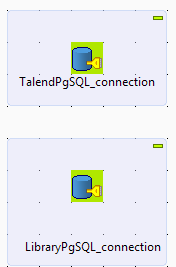
\includegraphics[scale=1]{images/db_connection.PNG}\\
La source CSV est toute aussi facile à configurer. Il suffit de configurer le séparateur, la présence ou non d'une entête et les colonnes à prendre en compte comme le montre la figure ci-dessous:\\

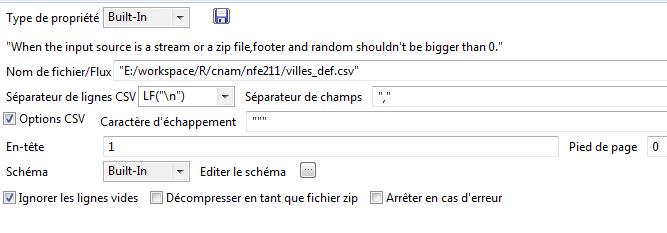
\includegraphics[scale=0.60]{images/csv.PNG}

\subsection{Dimension Boutique}
\subsubsection{Difficulté testée}
La difficulté ici est de lier des données entre deux sources de données de type différents : CSV et Database.

\subsubsection{Mise en œuvre}
Les deux sources de données configurées nous permettent de faire une jointure simple avec le composant tMap. Le lien entre les entités se fait de manière intuitive sur cet écran:

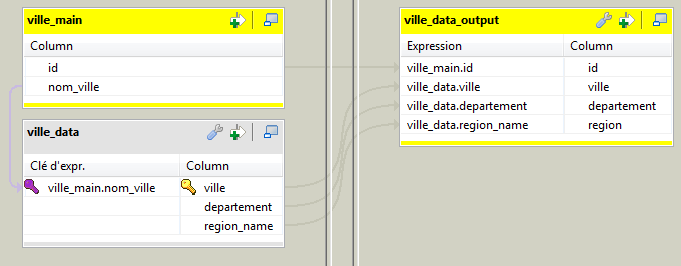
\includegraphics[scale=0.60]{images/ville_mappingcsv.PNG}\\
Dans la suite de ce projet nous utiliserons toujours une tMap pour faire une jointure entre deux sources de données.\\
Nous pouvons conclure que TALEND ne fait pas de distinction entre les différents types de données pourvu qu'elle soit composée de colonnes.

\subsection{Dimension Livre}
\subsubsection{Difficulté testée}
Aucune, jointure simple entre deux tables d'une base de données.

\subsubsection{Mise en œuvre}
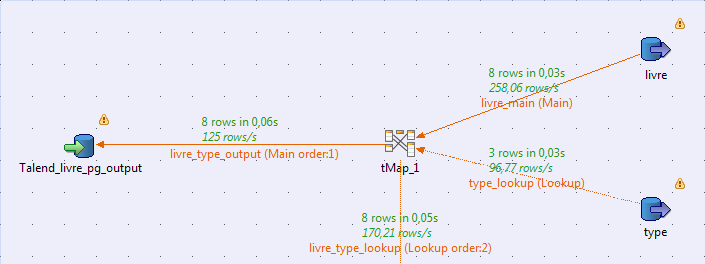
\includegraphics[scale=0.60]{images/dimension_livre.PNG}

\subsection{Dimension Client}
\subsubsection{Difficulté testée}
La dimension client est construite en utilisant la table client suivie d'une transformation sur l'un de ses champs afin de déduire la tranche d'age à partir de l'age.

\subsubsection{Mise en œuvre}
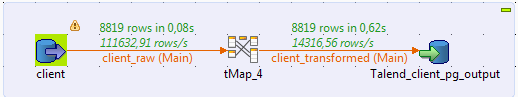
\includegraphics[scale=0.60]{images/dimension_client.PNG}\\

Pour transformer un age en tranche d'age, nous avons besoin de créer une routine dont le code est montré en annexe \ref{toTrancheDage} .

\subsection{Dimension Temps}
\subsubsection{Difficulté testée}
La dimension temps construite à partir de la table temps subit un action sur ses données afin d'enlever les doublons et de déterminer les hiérarchies à partir d'une date.
\subsubsection{Mise en œuvre}
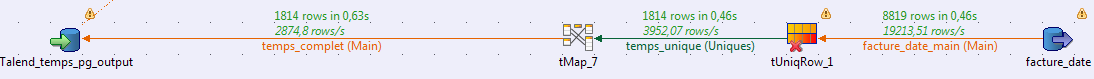
\includegraphics[scale=0.60]{images/dimension_temps.PNG}\\
Le composant tUniqRow\_ que nous voyons sur ce schéma sert à enlever les doublons. C'est à dire que nous voulons une seule date dans notre dimension temps. Nous prenons donc l'ensemble des dates distinctes trouvées dans la table facture.
Une fois ces dates trouvées, nous voulons déterminer les hiérarchies à partir du champs date\_achat de la table facture. Nous utilisons pour cela les fonctions built-in de TALEND :
\begin{itemize}
\item TalendDate.getPartOfDate("MONTH", date\_achat) pour déterminer le mois d'une date
\item TalendDate.getPartOfDate("YEAR", date\_achat)
\end{itemize}

\subsection{Table de faits vente}
\subsubsection{Difficulté testée}
Aucune, l'intégrité relationnelle des données est gérée côté base OLTP, ce qui réduit la création de la table de faits à un ensemble de jointure.
\subsubsection{Mise en œuvre}
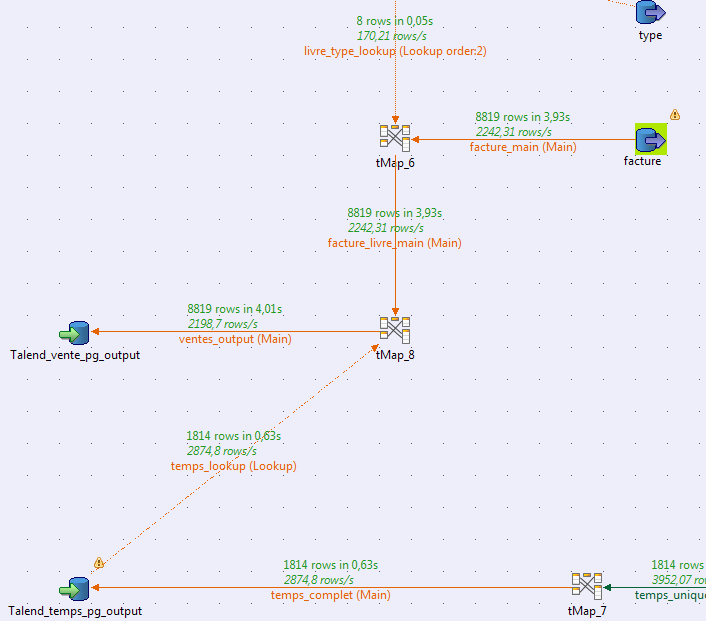
\includegraphics[scale=0.70]{images/table_faits_vente.PNG}

Aucune jointure avec la table client et la table boutique n'est nécessaire puisque les relations sont prises directement de la base OLTP et qu'aucune transormation sur les clés étrangères n'est effectuée.

\subsection{Conclusion sur l'utilisation de TALEND}
Pour les cas testés qui paraissent classiques, TALEND se montre plutôt efficace. La montée en charge reste à tester. Le nombre de composant paraît énorme et je n'ai pas réussi à les utiliser tous. C'est d'ailleurs un des défauts de TALEND à mon sens. L'utilisation n'est pas très intuitive et la résolution de problème est très compliquée. Lorsqu'un problème survient, l'utilisateur est gratifié d'un NullPointerException sans plus d'information. La modification du code JAVA généré est anecdotique selon moi même si son utilité est révélée lorqu'il s'agit de débugger. 
 
\clearpage
		
		\chapter{Le titre du chapitre}

\section{Le titre de la section qui va bien}

\subsection{Titre de la sous section}

Ici du texte et du blabla, ce que l'on veut dire et écrire. A remplacer. Ici du texte et du blabla, ce que l'on veut dire et écrire. On peut faire une citation \cite{Motclef1}.
A remplacer. Ici du texte et du blabla, ce que l'on veut dire et écrire. A remplacer. Ici du texte et du blabla, ce que l'on veut dire et écrire. A remplacer. Ici du texte et du blabla, ce que l'on veut dire et écrire. A remplacer. Ici du texte et du blabla, ce que l'on veut dire et écrire. A remplacer.

Ici du texte et du blabla, ce que l'on veut dire et écrire. A remplacer. Ici du texte et du blabla, ce que l'on veut dire et écrire. A remplacer.
Ici du texte et du blabla, ce que l'on veut dire et écrire. A remplacer. Ici du texte et du blabla, ce que l'on veut dire et écrire. A remplacer. Ici du texte et du blabla, ce que l'on veut dire et écrire. A remplacer. Ici du texte et du blabla, ce que l'on veut dire et écrire. A remplacer.

%-- Note de bas de page sur les stades
\protect\footnote{Par exemple, on peut faire un pied de page :
\begin{itemize}
\item avec une liste à puces ;
\item avec une liste à puces ;
\item avec une liste à puces.
\end{itemize}
}
%-- Fin Note de bas de page sur les stades

Ici du texte et du blabla, ce que l'on veut dire et écrire. A remplacer. Ici du texte et du blabla, ce que l'on veut dire et écrire. A remplacer. Ici du texte et du blabla, ce que l'on veut dire et écrire. A remplacer. Ici du texte et du blabla, ce que l'on veut dire et écrire. A remplacer. Ici du texte et du blabla, ce que l'on veut dire et écrire. A remplacer. Ici du texte et du blabla, ce que l'on veut dire et écrire. A remplacer.

\begin{itemize}
\item avec une liste à puces ;
\item avec une liste à puces ;
\item avec une liste à puces.
\end{itemize}

Ici du texte et du blabla, ce que l'on veut dire et écrire. A remplacer. Ici du texte et du blabla, ce que l'on veut dire et écrire. A remplacer. Ici du texte et du blabla, ce que l'on veut dire et écrire. A remplacer. Ici du texte et du blabla, ce que l'on veut dire et écrire. A remplacer. Ici du texte et du blabla, ce que l'on veut dire et écrire. A remplacer. Ici du texte et du blabla, ce que l'on veut dire et écrire. A remplacer.

\subsubsection{Titre de la sous sous section}

Ici du texte et du blabla, ce que l'on veut dire et écrire. A remplacer. Ici du texte et du blabla, ce que l'on veut dire et écrire. A remplacer. Ici du texte et du blabla, ce que l'on veut dire et écrire. A remplacer. Ici du texte et du blabla, ce que l'on veut dire et écrire. A remplacer. Ici du texte et du blabla, ce que l'on veut dire et écrire. A remplacer. Ici du texte et du blabla, ce que l'on veut dire et écrire. A remplacer.

Ici du texte et du blabla, ce que l'on veut dire et écrire. A remplacer. Ici du texte et du blabla, ce que l'on veut dire et écrire. A remplacer. Ici du texte et du blabla, ce que l'on veut dire et écrire. A remplacer. Ici du texte et du blabla, ce que l'on veut dire et écrire. A remplacer. Ici du texte et du blabla, ce que l'on veut dire et écrire. A remplacer. Ici du texte et du blabla, ce que l'on veut dire et écrire. A remplacer.

\subsubsection{Titre de la sous sous section}

Ici du texte et du blabla, ce que l'on veut dire et écrire. A remplacer. Ici du texte et du blabla, ce que l'on veut dire et écrire. A remplacer. Ici du texte et du blabla, ce que l'on veut dire et écrire. A remplacer. Ici du texte et du blabla, ce que l'on veut dire et écrire. A remplacer. Ici du texte et du blabla, ce que l'on veut dire et écrire. A remplacer. Ici du texte et du blabla, ce que l'on veut dire et écrire. A remplacer.

Ici du texte et du blabla, ce que l'on veut dire et écrire. A remplacer. Ici du texte et du blabla, ce que l'on veut dire et écrire. A remplacer. Ici du texte et du blabla, ce que l'on veut dire et écrire. A remplacer. Ici du texte et du blabla, ce que l'on veut dire et écrire. A remplacer. Ici du texte et du blabla, ce que l'on veut dire et écrire. A remplacer. Ici du texte et du blabla, ce que l'on veut dire et écrire. A remplacer.

\subsection{Conclusion}

Ici du texte et du blabla, ce que l'on veut dire et écrire. A remplacer. Ici du texte et du blabla, ce que l'on veut dire et écrire. A remplacer. Ici du texte et du blabla, ce que l'on veut dire et écrire. A remplacer. Ici du texte et du blabla, ce que l'on veut dire et écrire. A remplacer. Ici du texte et du blabla, ce que l'on veut dire et écrire. A remplacer. Ici du texte et du blabla, ce que l'on veut dire et écrire. A remplacer.

Ici du texte et du blabla, ce que l'on veut dire et écrire. A remplacer. Ici du texte et du blabla, ce que l'on veut dire et écrire. A remplacer. Ici du texte et du blabla, ce que l'on veut dire et écrire. A remplacer. Ici du texte et du blabla, ce que l'on veut dire et écrire. A remplacer. Ici du texte et du blabla, ce que l'on veut dire et écrire. A remplacer. Ici du texte et du blabla, ce que l'on veut dire et écrire. A remplacer.

\subsection{Titre de la sous section}

Ici du texte et du blabla, ce que l'on veut dire et écrire. A remplacer. Ici du texte et du blabla, ce que l'on veut dire et écrire. On peut faire une citation \cite{Motclef1}.
A remplacer. Ici du texte et du blabla, ce que l'on veut dire et écrire. A remplacer. Ici du texte et du blabla, ce que l'on veut dire et écrire. A remplacer. Ici du texte et du blabla, ce que l'on veut dire et écrire. A remplacer. Ici du texte et du blabla, ce que l'on veut dire et écrire. A remplacer.

Ici du texte et du blabla, ce que l'on veut dire et écrire. A remplacer. Ici du texte et du blabla, ce que l'on veut dire et écrire. A remplacer.
Ici du texte et du blabla, ce que l'on veut dire et écrire. A remplacer. Ici du texte et du blabla, ce que l'on veut dire et écrire. A remplacer. Ici du texte et du blabla, ce que l'on veut dire et écrire. A remplacer. Ici du texte et du blabla, ce que l'on veut dire et écrire. A remplacer.

\subsection{Titre de la sous section}

Ici du texte et du blabla, ce que l'on veut dire et écrire. A remplacer. Ici du texte et du blabla, ce que l'on veut dire et écrire. On peut faire une citation \cite{Motclef1}.
A remplacer. Ici du texte et du blabla, ce que l'on veut dire et écrire. A remplacer. Ici du texte et du blabla, ce que l'on veut dire et écrire. A remplacer. Ici du texte et du blabla, ce que l'on veut dire et écrire. A remplacer. Ici du texte et du blabla, ce que l'on veut dire et écrire. A remplacer.

Ici du texte et du blabla, ce que l'on veut dire et écrire. A remplacer. Ici du texte et du blabla, ce que l'on veut dire et écrire. A remplacer.
Ici du texte et du blabla, ce que l'on veut dire et écrire. A remplacer. Ici du texte et du blabla, ce que l'on veut dire et écrire. A remplacer. Ici du texte et du blabla, ce que l'on veut dire et écrire. A remplacer. Ici du texte et du blabla, ce que l'on veut dire et écrire. A remplacer.

\clearpage


		\chapter{Conclusion}

La chaine décisionnelle telle que proposée en introduction est intéressante pour l'exercice mais ne semble pas être la plus optimale pour une utilisation industrialisée en entreprise. \\
Pour la partie TALEND, j'aimerai tester l'intégration du jar générable dans une application JEE ou tout simplement lancé par un ordonnanceur en batch quotidien. La montée en charge du jar généré doit être intéressante à évaluer aussi. Le fait qu'il s'agisse de JAVA rend possible l'investigation par des experts JAVA notamment à l'aide d'outil de profiling. Même si l'expérience utilisateur a été pour moi désastreuse, je ne l'éliminerai pas d'un choix à faire en entreprise sans évaluation et confrontation au besoin.\\
L'utilisation de SAS pour la partie reporting ne m'a pas convaincue. Soit je suis passé à côté, soit l'outil semble dédié à un besoin très particulier qui le ferait exclure de nombreuses études de mise en place d'outil de reporting. L'outil semble destiné à des développeurs SAS ayant surtout besoin d'une capacité à traiter d'éléments statistiques sur de grands volumes de données. Chose que je n'ai pas testée. Je ne pense pas qu'il soit destiné à des décideurs à part évidemment les rapports produits.


		% Pour finir l'interligne de 1,5
	\end{onehalfspace}


\appendix

	\begin{onehalfspace}
\chapter{Annexes}
\section{Code R ayant généré les données}\label{generateDataR}
\lstset{language=java}
\lstset{frame=shadowbox}
\lstinputlisting[caption=generateData.R]{./texte/client.R}

\clearpage

\section{Routine java toTrancheDage.java}\label{toTrancheDage}

\lstset{language=java}
\lstset{frame=shadowbox}
\lstinputlisting[caption=toTrancheDage.java]{./texte/toTrancheDage.java}

\section{import.sas}\label{import.sas}

\lstset{language=sql}
\lstset{frame=shadowbox}
\lstinputlisting[caption=import.sas]{./texte/import.sas}

\section{reporting.sas}\label{reporting.sas}

\lstset{language=sql}
\lstset{frame=shadowbox}
\lstinputlisting[caption=reporting.sas]{./texte/reporting.sas}

\section{report sas}\label{reporting-results}
%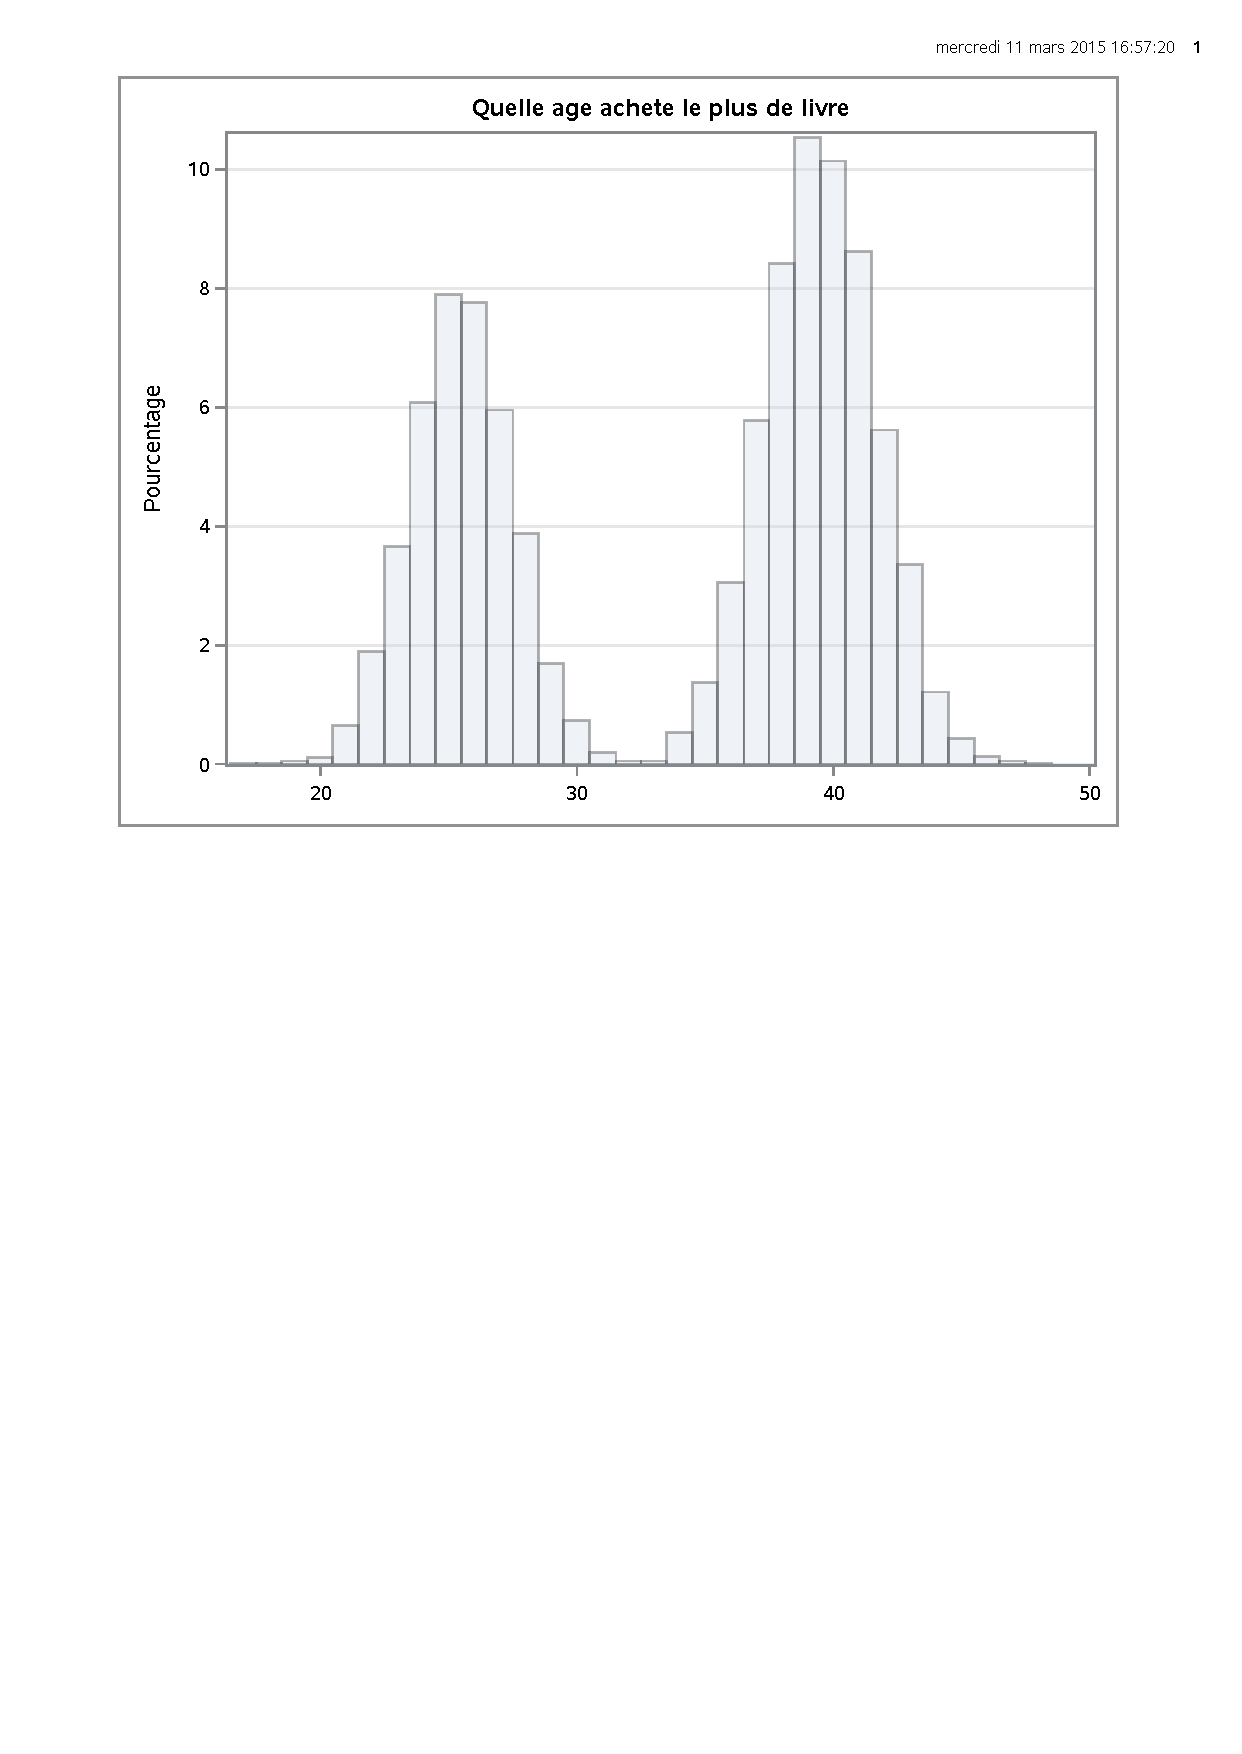
\includepdf[pages={-}]{./texte/reporting.pdf}
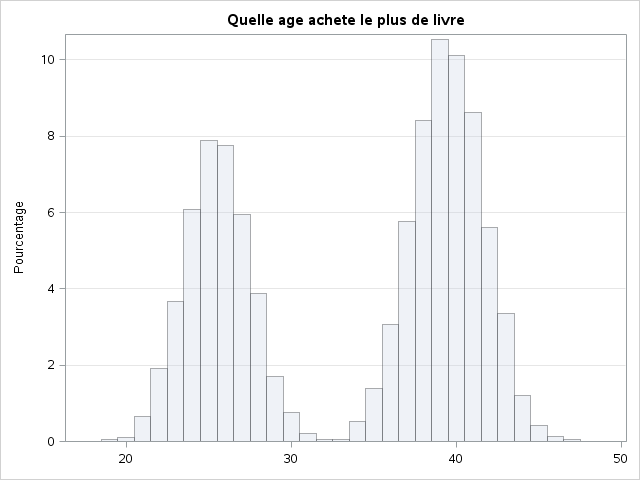
\includegraphics[scale=0.7]{./images/sas_report/age_vente_livre.png}
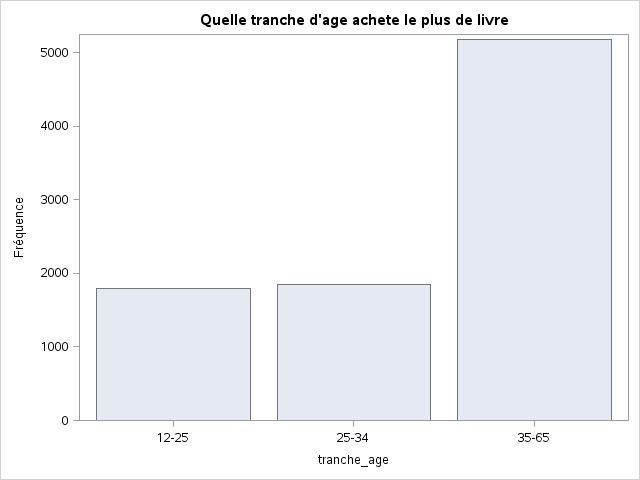
\includegraphics[scale=0.7]{./images/sas_report/tranche_age_livre.png}
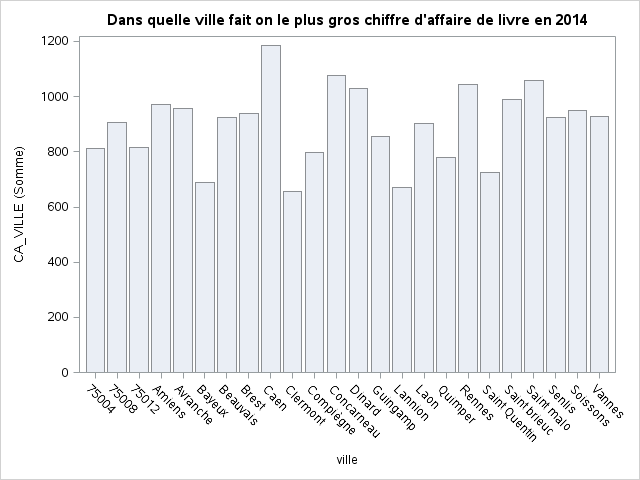
\includegraphics[scale=0.7]{./images/sas_report/ville_2014.png}
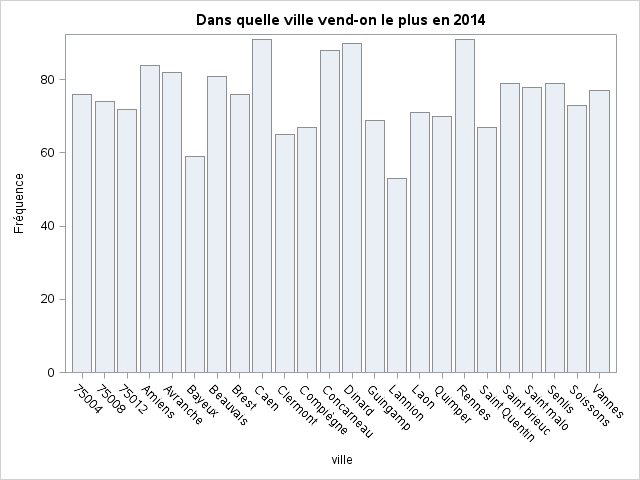
\includegraphics[scale=0.7]{./images/sas_report/ville_2014-frequence.png}
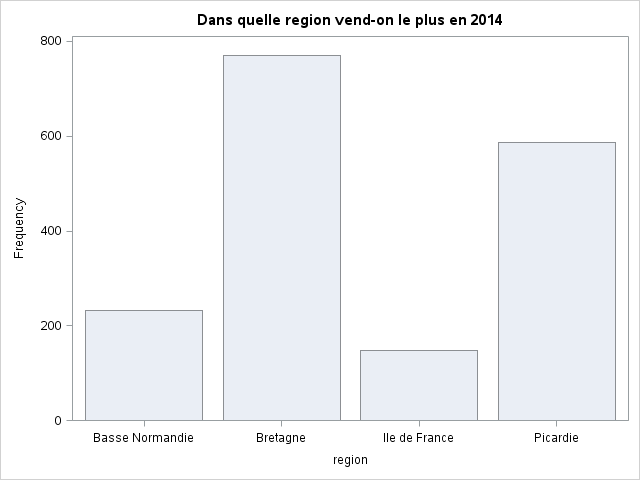
\includegraphics[scale=0.7]{./images/sas_report/region_2014.png}
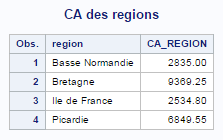
\includegraphics[scale=0.7]{./images/sas_report/table_sas.PNG}
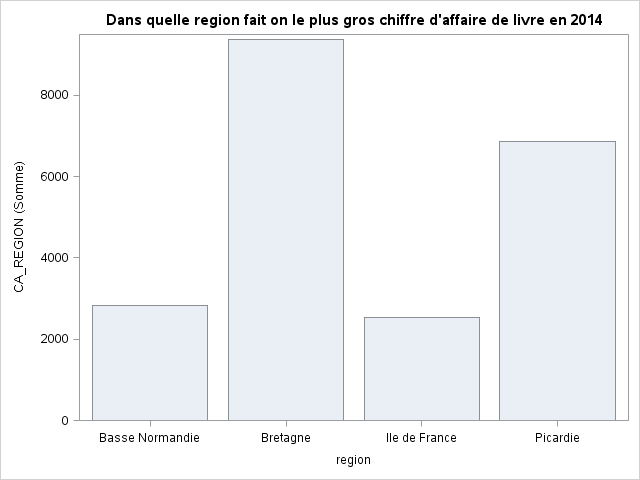
\includegraphics[scale=0.7]{./images/sas_report/nb_ville_region.png}
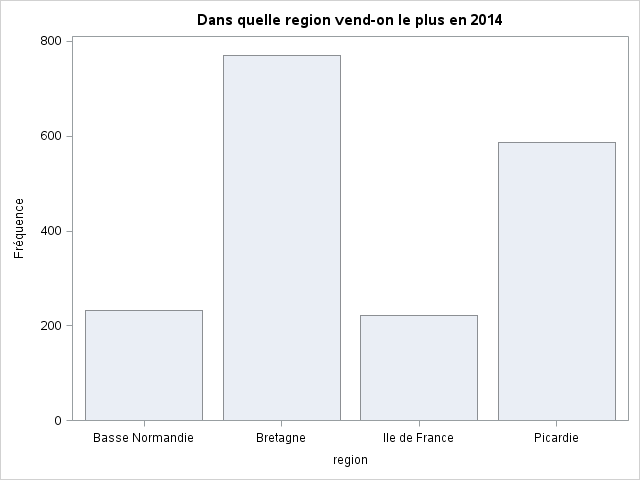
\includegraphics[scale=0.7]{./images/sas_report/sas_report_1.png}
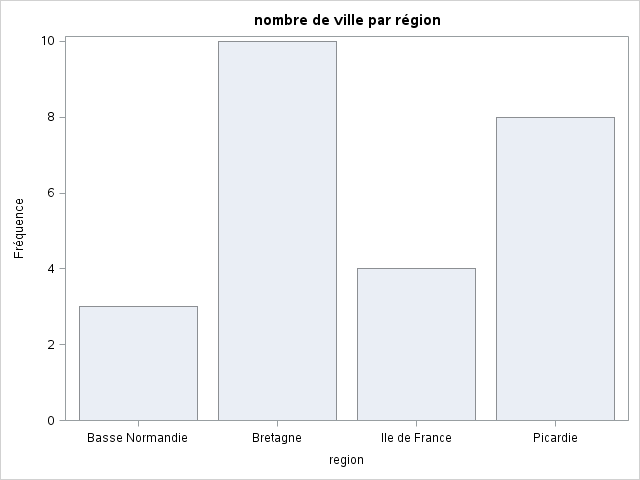
\includegraphics[scale=0.7]{./images/sas_report/sas_report_2.png}
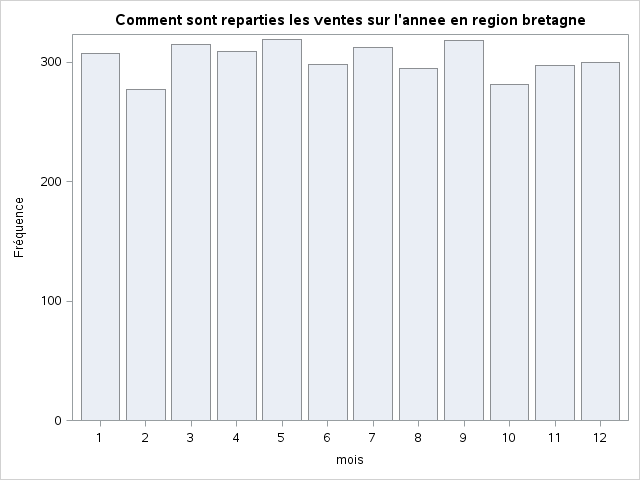
\includegraphics[scale=0.7]{./images/sas_report/sas_report_3.png}
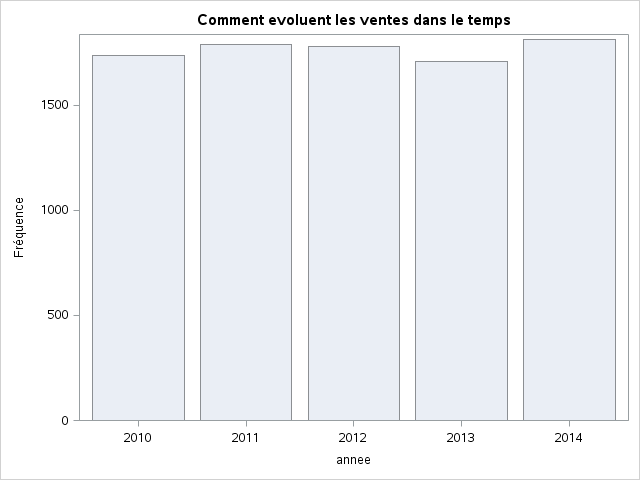
\includegraphics[scale=0.7]{./images/sas_report/sas_report_4.png}
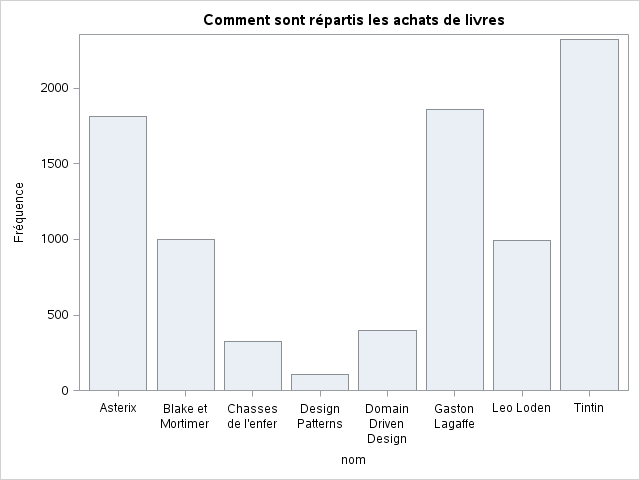
\includegraphics[scale=0.7]{./images/sas_report/sas_report_5.png}
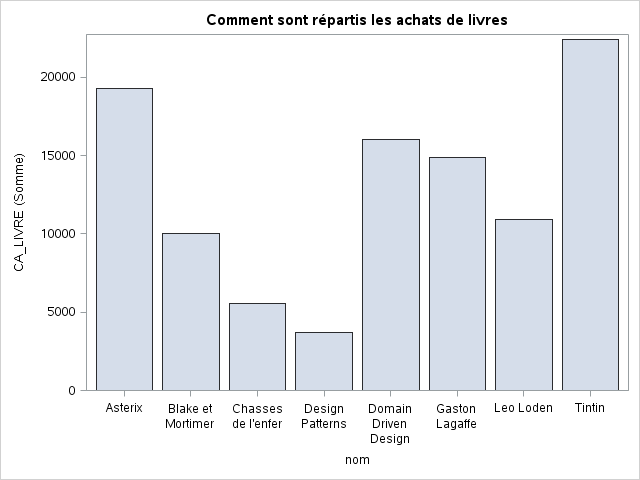
\includegraphics[scale=0.7]{./images/sas_report/sas_report_6.png}
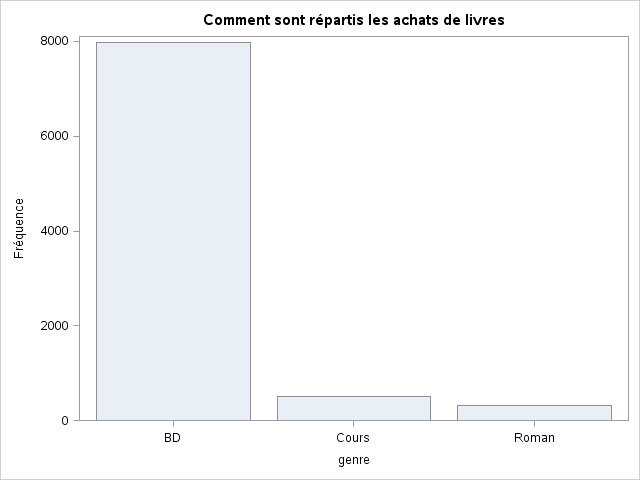
\includegraphics[scale=0.7]{./images/sas_report/sas_report_7.png}
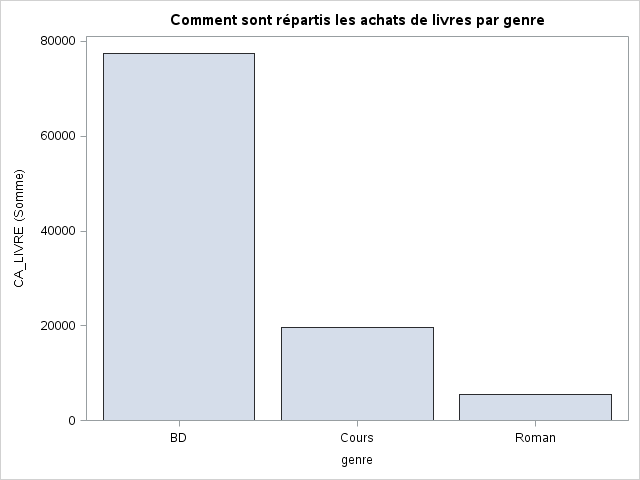
\includegraphics[scale=0.7]{./images/sas_report/sas_report_8.png}
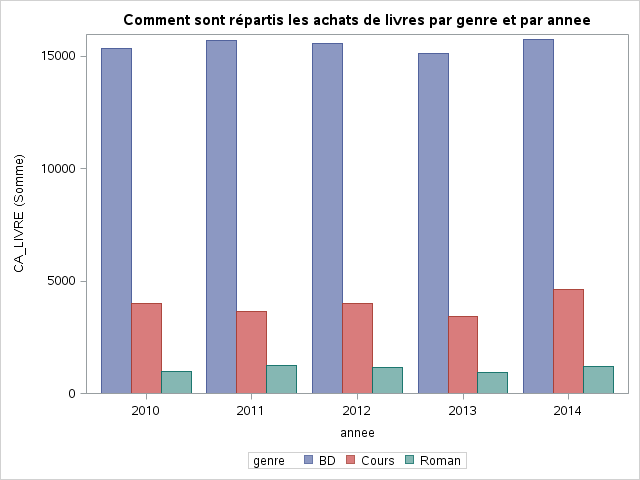
\includegraphics[scale=0.7]{./images/sas_report/sas_report_9.png}

		% Pour finir l'interligne de 1,5
	\end{onehalfspace}





%----------------------------------------
% Pour la bibliographie


% Citer tous les ouvrages/références
\nocite{*}
% Trier par ordre d'apparition
%\bibliographystyle{unsrt}
% Pour le style de la biblio
\bibliographystyle{plain}
% Ecrire la biblio ici
\bibliography{biblio}

\printindex

\end{document}
